\documentclass{article}
\usepackage {graphicx}
\begin{document}
\title{Machine, Data and Learning: Assignment 1}
\author{Shubhangi Dutta (2018113004), Rishav Kundu (2019121007)}
\maketitle
\newpage
\section{Bias and Variance}
The formula for bias is given as 
\newline
$$Bias=(E[\hat{f}(x)]-f(x))$$
\newline 
Therefore, 
\newline
$$
Bias^2=(E[\hat{f}(x)]-f(x))^2
$$
\newline
The formula for variance is given as 
$$
Variance=E[\hat{f}(x)-E[\hat{f}(x)])^2]
$$
The above formulas are defined for a single value of $x$. Hence, the expectation $E[\hat{f}(x)]$ is defined over the different values of $\hat{f}(x)$ obtained by training the same model on different training set partitions.
\section{Q1}
\subsection{Bias and Variance table for Polynomial Fit}

\begin{center}
\begin{tabular}{ | c | c | c | }
\hline
Degree & Bias & Variance \\ 

\hline
1 & 5.615473846158311 & 0.16798807712862038 \\
\hline
2 & 2.4162068154669063 & 0.04000493893369631 \\
\hline
3 & 2.215722594768818 & 0.04900029595191231 \\
\hline
4 & 1.7616085631225642 & 0.03247952144688806 \\
\hline
5 & 1.7446521530578816 & 0.03272471210065929 \\
\hline
6 & 1.616260750124133 & 0.03479236574895368 \\
\hline
7 & 1.5694763199132815 & 0.03840954023428789 \\
\hline
8 & 1.552554208565159 & 0.044894310009533166 \\
\hline
9 & 1.5488808680984325 & 0.04563749022029945 \\
\hline
10 & 1.546901886043299 & 0.048901753121171884 \\
\hline
11 & 1.5002602307899762 & 0.04262705768129397 \\
\hline
12 & 1.5002026543610982 & 0.04774657665384174 \\
\hline
13 & 1.440494706432324 & 0.04888148723035307 \\
\hline
14 & 1.442563667859875 & 0.05429555689868246 \\
\hline
15 & 1.4392894855480474 & 0.05485541993113892 \\
\hline
16 & 1.4404513259931004 & 0.05610690544072101 \\
\hline
17 & 1.4447416013608068 & 0.05510355831386975 \\
\hline
18 & 1.4505998513262797 & 0.05331434847877483 \\
\hline
19 & 1.4455573853067498 & 0.05060368021809415 \\
\hline
20 & 1.4391479363858821 & 0.05005170375681526 \\
\hline
21 & 1.4395406482226982 & 0.04736032951518309 \\
\hline
22 & 1.448308754071106 & 0.053069921804461406 \\
\hline
23 & 1.4514879619950398 & 0.048098456745089085 \\
\hline
24 & 1.4606394099272366 & 0.04711157128242785 \\
\hline
25 & 1.454877703295114 & 0.042508364535212166 \\
\hline
26 & 1.4914170182126254 & 0.06074501206927735 \\
\hline
27 & 1.533693743464152 & 0.049086056290609366 \\
\hline
28 & 1.5652070154715143 & 0.042138036739928955 \\
\hline
29 & 1.595128629167355 & 0.03444974768324535 \\
\hline
30 & 1.6214225829486661 & 0.028618478909667507 \\
\hline
\end{tabular}
\end{center}

\subsection{Bias-Variance Vs Degree Plot for Polynomials Degree 1-9}
\subsubsection{Plot}
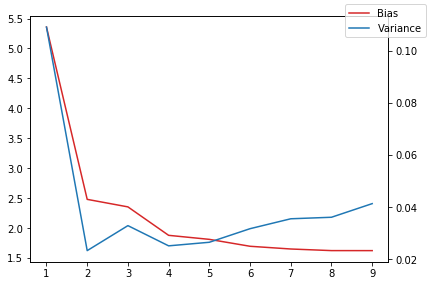
\includegraphics[scale=.9]{images/1-9.png}
\subsubsection{Observations and Analysis}
\begin{itemize}
\item Both bias and variance are very large for the linear fit. The model is underfit and performs poorly for the given data.
\item For higher degrees ($>$1, $<$ 6), both bias and variance decrease. The models are better fit to the data points, so both decrease.
\item Variance increases again for even higher degree polynomials ($>$6) but it is not significant compared to the drop between degree  1 and 2. The model is overfitting, and hence is not a good fit for the test data and is accounting for small deviations, making variance high.
\end{itemize}
\subsection{Bias-Variance Vs Degree Plot for Polynomials Degree 2-9}
We remove the first point to better view the changes between the other degrees.
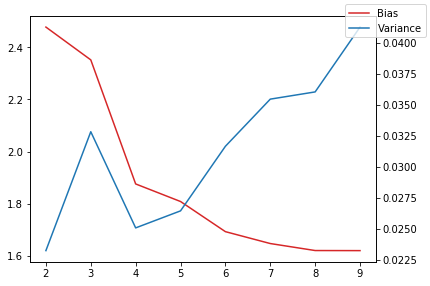
\includegraphics[scale=.9]{images/2-9.png}
\subsubsection{Observations and Analysis}
\begin{itemize}
\item Bias is high but variance is low for the degree 2 fit. The model is underfit and performs poorly for the test data.
\item For higher degrees ($>$ 2, $<$ 5), both bias and variance decrease. The models are better fit to the data points, so both decrease.
\item The intersection point is at the 5 degree polynomial. Both bias and variance are low and this is optimal fit.
\item Variance increases again for even higher degree polynomials ($>$6) and it is significant compared to the drop in bias. The model is overfitting, and hence is not a good fit for the test data and is accounting for small deviations, making variance high.
\end{itemize}
\subsection{Bias-Variance Vs Degree Plot for Polynomials Degree 1-30}
We increase the degree of the polynomial to get a wider view of the data.
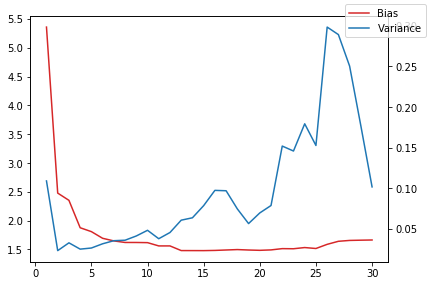
\includegraphics[scale=.9]{images/1-30.png}
\subsubsection{Observations and Analysis}
\begin{itemize}
\item Both bias and variance are very large for the linear fit. The model is underfit and performs poorly for the given data.
\item For higher degrees ($>$ 1, $<$ 10), both bias and variance decrease. The models are better fit to the data points, so both decrease.
\item The intersection point is at the 5 degree polynomial. Both bias and variance are low and this is optimal fit.
\item Variance increases again sharply for even higher degree polynomials (>10). Bias keeps reducing in approximately linear way. The model is overfitting, and hence is not a good fit for the test data and is accounting for small deviations, making variance high. 
\item In some cases, such as at degree 24-25 and again at 30. In these cases, the model incidentally fit well, probably due to the nature of the data.
\end{itemize}

\section{Q2}
\subsection{Bias and Variance table for Polynomial Fit}
\begin{center}
\begin{tabular}{ | c | c | c | }
\hline
Degree & Bias & Variance \\
\hline
1 & 999.6141239858127 & 70545.48914575046 \\
\hline
2 & 977.0461983931082 & 125870.85554877334 \\
\hline
3 & 96.90061979570203 & 150073.7395464768 \\
\hline
4 & 104.43825033995597 & 212235.70832526154 \\
\hline
5 & 96.63950688681115 & 276388.48025474057 \\
\hline
6 & 101.23529987681114 & 316863.49843748985 \\
\hline
7 & 101.66255879943755 & 357510.98475735466 \\
\hline
8 & 100.74432611287484 & 404286.670685786 \\
\hline
9 & 103.99753380044281 & 459132.37837248633 \\
\hline
\end{tabular}
\end{center}
\subsection{Bias-Variance Vs Degree Plot for Polynomials Degree 1-9}
\subsubsection{Plot}
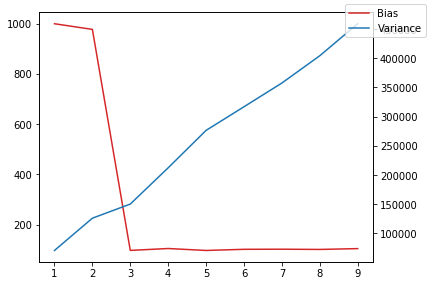
\includegraphics[scale=.9]{images/1-9-2.png}
\subsubsection{Observations and Analysis}
\begin{itemize}
\item Both bias and variance are very large for the linear fit. The model is underfit and performs poorly for the given data.
\item For higher degrees ($>$1, $<$3), both bias and variance decrease. The models are better fit to the data points, so both decrease.
\item Variance increases again for even higher degree polynomials ($>$3) but it is not significant compared to the drop between degree  1 and 2. The model is overfitting, and hence is not a good fit for the test data and is accounting for small deviations, making variance high.
\end{itemize}
\subsection{Bias-Variance Vs Degree Plot for Polynomials Degree 3-9}
We remove the first point to better view the changes between the other degrees.
\subsubsection{Plot}
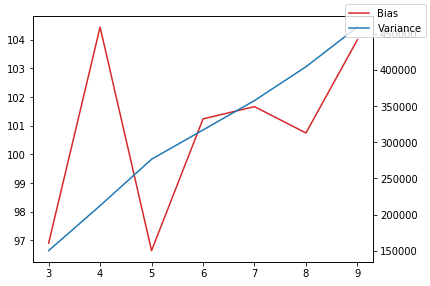
\includegraphics[scale=.9]{images/3-9.png}
\subsubsection{Observations and Analysis}
\begin{itemize}
\item Both bias and variance are very low for the 3 degree fit. The model is a better fit for the data.
\item For higher degrees ($>$3), both bias and variance increase. The training data has a lot of noise, hence they increase the bias and the variance both.
\item Variance increases again for even higher degree polynomials ($>$6). The model is overfitting, and hence is not a good fit for the test data and is accounting for small deviations, making variance high.
\end{itemize}
\subsection{Analysis of Data given}
From the above observations, we can see that the test data is very noisy compared to the training data. Hence the bias and variance are both high at the linear fit, and then reach a minimum at the degree 3. The higher degree models try to acount for the noise and both bias and variance become higher.

\subsubsection{Plot of Training Data}
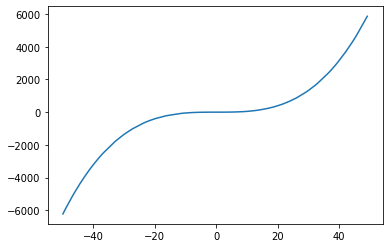
\includegraphics[scale=.9]{images/train-2.png}

We see that a three degree fit is the best fit for the training data.


\subsubsection{Plot of Test Data}
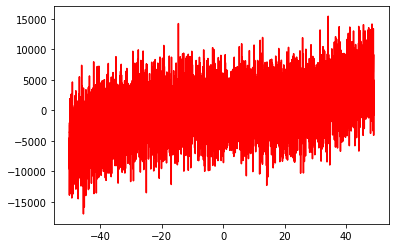
\includegraphics[scale=.9]{images/test-2.png}

We see that the test data is very noisy compared to the training data, which explains the high bias and variance.

\end{document}
